\documentclass[11pt]{article}

\usepackage{fullpage}
\usepackage{graphicx}
\usepackage{hyperref}
\usepackage{booktabs}
\usepackage{float}
\usepackage[linesnumbered,ruled,vlined]{algorithm2e}
\usepackage{amsmath}


\title{Improved Multi-Agent Knowledge Sharing System using Knowledge Graphs for News Bias Detection and Fact-Checking}

\author{Modupeola Fagbenro$^{1}$, Christopher Washer$^{1}$, Pavani Chella$^{1}$, and Amir Jafari$^{1}$,\\
\small $^{1}$Department of Data Science, The George Washington University, Washington, DC, USA\\
\small \texttt{modupeola.fagbenro@gwu.edu, cwasher@gwu.edu, pavani.chella@gwu.edu,ajafari@gwu.edu}
}
\date{} %don't display the current date


\begin{document}

\maketitle

\begin{abstract}

This research study explores how integrating a multi-agent system with a knowledge graph as shared memory enhances news bias analyses, detection, and fact-checking. Automated fact-checking and verification systems have evolved significantly but often struggle with complex contextual information and advanced narratives. This research investigates improving accuracy, precision, and recall when multi-agent systems incorporate knowledge graphs compared to systems without knowledge graph integration.  This system was designed and implemented as a framework in which multiple specialized agents using Large Language Models (LLMs) collaborate while building and referencing a shared knowledge graph. Experiments conducted on diverse political news article datasets show that integrating knowledge graphs improved performance over an LLM alone, with bias detection balance accuracy from 0.735 to 0.823 and fact-checking precision from 0.75 to 0.78. These findings suggest that integrating a knowledge graph into a multi-agent system provides the context needed to improve reasoning for media bias detection and fact-checking.

  
\end{abstract}

\section{Introduction}
\subsection{Background}

\subsubsection{\textbf{Misinformation and Media Bias In The News Landscape}}

Misinformation and bias in the news media are widespread issues in today's digital media landscape, with real societal implications. Misinformation refers to false, misleading, or inaccurate information spread (intentional or not), proliferating rapidly on social media. The ease of producing and sharing content online leads to false information reaching millions, which makes it a significant threat to public interests \cite{r1}.
Filling social media feeds with misleading claims can confuse and overwhelm the public and erode trust in institutions and elections \cite{r2}. Examples such as false stories about the 2020 U.S. presidential election suggest that misinformation can impact political outcomes. The issue is well known enough that over half of Americans expect political misinformation to worsen in their lifetimes, highlighting the increasing prevalence of this problem \cite{r3}\cite{r4}. 
Media bias refers to partiality in news reporting through tone, framing, or story selection that skews information in favor of a particular viewpoint. News media bias often results in audiences self-selecting news sources that support their existing beliefs, and the sources can reinforce them by presenting information through a partisan lens. Over time, biased presentation and consumption can produce different versions of reality for different audiences.
A recent study of Breitbart, a conservative news outlet, and the New York Times, a left-leaning news outlet, found that each outlet was relatively neutral in coverage, but exhibited a polarizing attitude towards specific entities, contributing to disparities in audience political views \cite{r5}. This finding supports similar work looking at these two news outlets, showing how changes to similar common words can impart a different meaning to their audiences \cite{r6}. Therefore, even when mainstream outlets aim for accuracy, selective emphasis on certain topics or certain word choices can reinforce political polarization. Continued research is needed to counter these trends in media bias and misinformation to improve the political news landscape.

\subsubsection{Knowledge graphs in information processing}

Knowledge graphs (KGs) are a structured way of representing and organizing complex information using a network of nodes (entities such as people, organizations, events, or concepts) and edges (relationships between those entities), typically expressed as subject-predicate-object triplets \cite{r7}. This structure allows information to be stored in a way that mirrors real-world relationships.: For example, a KG can represent the fact that a politician belongs to a specific political party with the triplet:' Politician - memberOf - party'. These triplets allow for context-rich storing of information as the connections between nodes model the logic and structure of content. Linking discrete data points into a graph enables structure-based and semantic reasoning by traversing nodes and connections to infer new insight or answer complex queries \cite{r8}. Unlike unstructured text or relational databases, the interconnected structure of a KG supports advanced retrieval and inference.

KGs are integral to many complex information systems that require access to structured knowledge \cite{r9}. Search engines use massive KGs (such as Google Knowledge Graph) to enrich search results. In the context of news and fact-checking, KGs offer a way to compile and link vast amounts of information about entities, claims, and sources. A news oriented KG can connect a claim to who said it and what evidence supports or refutes it, enabling automated reasoning about truthfulness\cite{r10}.
For bias detection, a KG can represent a network of articles with source or political bias information and help identify patterns such as grouping articles that frame an event similarly. A recent study built a political KG and showed that it improved political perspective detection in news media \cite{r11}. The KG provided structured context from real-world political dynamics that are missing in similar text-only models, highlighting how KGs can aid processing tasks by providing broader factual and relational content.

 





\subsection{Problem Statement}
\subsubsection{Challenges in news evaluation }


Evaluating news for bias and misinformation is a difficult task, with human and computational limitations. One major challenge is the daily number of news articles and social media claims that emerge outpaces what human fact-check teams or editors can feasibly review. Studies find that professional fact-checkers may spend hours on a given claim, making purely manual verification insufficient against the increasing tide of online information \cite{r12}. This leads to a verification delay; by the time a human analysis is complete and published, the misinformation may already be widely spread. Bias may often be complicated by the reader; what one person perceives as biased, another might view as reasonable, making it difficult for ground truth bias detection.
Automated approaches have other difficulties. Automated bias detection is challenging because bias can be nuanced: it may appear through tone, omission of context, or choice of sources, which require understanding beyond surface text features. Early machine learning models often picked up on spurious signals; for example, a classifier could mainly learn the source publication as a proxy for bias without analyzing the content \cite{r13}. This limitation often reduces generalizability for new or moderate outlets.


Automated fact-checking has similar challenges, as natural language processing-based approaches lack world knowledge and context to spot subtle misinformation or biases. Traditional models check if phrasing or metadata resembles known false statements and might struggle without contextual knowledge. Modern large language models (LLMs) bring in-depth language understanding, but despite this methodology, they still suffer from hallucinations and produce confident-sounding but incorrect answers\cite{r14}. LLMs are constrained by what they have seen in training, so recent research is often not in their knowledge base, which is essential for news-based fact-checking.
 
\subsubsection{Need for automated fact-checking and bias detection}
Given these challenges, there is a clear need for automated approaches to assist in fact-checking and bias detection. No newsroom or fact-checking team can keep up with the influx of online claims, so scalable AI agents are needed to help monitor and evaluate content \cite{r12}. Automated systems can rapidly flag potential misinformation or extreme bias for news teams to review. While automation is essential, it is important to combine it with robust knowledge resources to improve accuracy. By connecting LLM-based agents to an external KG, we can ground their analysis in up-to-date, verified information. The LLM brings comprehension and reasoning, while the KG provides retrievable evidence that the LLM can use to make informed judgments.
Overall, the high volume of content, the nuance of bias detection, and the knowledge limitations of artificial intelligence make news evaluation a difficult problem. For these reasons we suggest that KG-integrated multi-agent systems offer an improved approach to combating misinformation and media bias over traditional or LLM-only methods.  



\subsection{Research Objectives}
\subsubsection{Primary objectives}

\begin{enumerate}
    \item Assess the impact of shared KG-based memory in a multi-agent system on news bias detection and fact-checking accuracy.

    \item Measure the performance difference between multi-agent systems with and without KG integration to show the effect a KG can have in addressing complex news evaluation tasks.
\end{enumerate}

\subsubsection{Specific research questions}

\begin{enumerate}
    \item What is the impact of knowledge graph integration into multi-agent system capabilities in bias detection, fact-checking, and overall system evaluation?
\end{enumerate}


\subsection{Dataset Description}
\subsubsection{Source and characteristics}

The news KG integration to support this system was constructed from a comprehensive corpus of political articles collected via the NewsAPI aggregator \cite{r15}. We focused on a curated list of 20 well-known news outlets spanning the ideological spectrum, including ABC News, Associated Press, Axios, Breitbart News, CBS News, CNN, Fox News, MSNBC, National Review, NBC News, Newsweek, New York Magazine, Politico, Reuters, The American Conservative, The Hill, The Huffington Post, The Washington Post, The Washington Times, and USA Today. These sources were selected to ensure a balance of political leanings and editorial standards. Each source’s known bias was characterized using ratings from AllSides \cite{r16}, which provides crowd-sourced reviews augmented by expert editorial analysis. AllSides’ media bias classification (on a three-point left-center-right scale) was used for the political bias of each source, and this metadata was associated with the corresponding source and article entries in the knowledge graph.

For fact checking, we compiled a benchmark data set by scraping the Daily Fact Checks of Media Bias / Fact Check (MBFC)\cite{r17}. MBFC publishes daily summaries of fact checks drawn from internationally recognized fact-checking organizations. For bias detection, a separate corpus of articles was assembled, each article labeled according to its source’s AllSides bias rating. This data set reflects a mix of left, center, and right biases based on the outlet of origin, serving as ground truth for testing the bias detection capabilities of the system. 



\subsection{Research Implications and Contributions}
\subsubsection{Theoretical contributions}
\begin{enumerate}
    \item This research shows integrating a shared KG into a multi-agent system creates measurable performance improvements in complex news evaluation tasks.
        \item This research serves as a framework for agent collaboration through the use of a shared knowledge graph database.
\end{enumerate}

\subsubsection{Practical applications}
\begin{enumerate}
    \item This system and the methods explored can be used by fact-check or editorial teams to assist in media evaluation. News consumers can also benefit from the increased transparency our system offers. 
    \item Educators and independent news outlets can use this system to demonstrate media bias and misinformation in the US political domain. 


\end{enumerate}

\section{Related Work and Literature Review}
\subsubsection{Existing News Evaluation Systems}
In response to increasing misinformation, platforms such as Ground News\cite{r18} and AllSides use comparative bias tracking to analyze stories across various political media outlets. These platforms give news consumers an understanding of the of the bias associated with sources and news coverage but may not address individual news articles or independent media sources. 

Academic researchers have proposed solutions employing natural language processing to evaluate factual accuracy and bias\cite{r19}. While this effectively detects coverage discrepancies, they have often faced a problem operating in isolation.  This research provides groundwork for automated bias detection and fact checking but does not do so in a multi-agent collaborative fashion which may limit the overall functionality in real world application.

\subsubsection{Multi-Agent Architectures}
Multi-agent systems have become popular in knowledge-intensive domains because of their modularity and distributed problem-solving capabilities. Multi-agent systems were created as a framework for agent autonomy in foundational research work \cite{r20}. Recent studies have shown the effectiveness of implementing large language models (LLMs) as the decision makers and operators\cite{r21}\cite{r22}. These system architectures, orchestrated by platforms like LangChain\cite{r23}, facilitate shared memory and modular reasoning among agents, enhancing their collaborative interaction. Despite ongoing advanced research, there is limited application of integrating these systems with a shared knowledge graph-based memory or applying them to news evaluation tasks.

\subsubsection{Knowledge Graph Applications in Information Processing}
KGs are fundamental in structured information representation with semantically enriched storage for entity-relation triplets. KGs often used enable the connection of diverse news topics and sources through semantic reasoning and logic. Tools like Neo4j have robust capabilities designed to make them more suitable for dynamic, evolving datasets such as political news. Recent initiatives \cite{r24}\cite{r25}investigate the integration of knowledge graphs with transformer-based models to improve claim verification and event linking. However, building a KG to support a multi-agent setting in this domain, remains unexplored.

\subsubsection{Fact-Checking Methodologies}
Fact-checking is a popular area of research for the application of LLM-based systems.  Approaches have progressed from simple binary verification to  more complex, context-sensitive analysis. Recent methodologies utilize transformer-based models trained on datasets such as LIAR\cite{r26} and BABE \cite{r27}, while earlier research findings in similar systems, like ClaimBuster \cite{r28}, implemented rule-based filters and similarity metrics \cite{r29}. Recent advancements have explored chaining together multiple facts through multi-hop reasoning and entailment analysis to verify claims\cite{r30}. Nonetheless, there are still concerns regarding hallucinations in outputs generated by large language models, the weighting of source credibility, and scalability across various human domains and languages. The integration of a structured memory via KG into a fact-checking processes is a promising opportunity to improve on past in verification workflows.

\subsubsection{Bias Detection Approaches}
The identification of bias in news includes story selection, tone, or choice of sources. Linguistic models have been trained to recognize subjective words, sentiment polarity, and modality \cite{r31}. Recent efforts leverage models which account for political alignment, narrative framing, and language cues\cite{r32}. LLMs fine-tuned on news bias-related corpora have demonstrated improvement in bias detection, particularly when paired with external contextual data.


\subsubsection{Research Gaps and Opportunities}

There are of a growing number tools and methodologies in the domain of news evaluation but various limitations and setbacks have slowed advancement. First, effective solutions often work in  isolation lacking the collaborative nature multi-agent system designs. Second, while KGs offer semantic depth, their integration with agent-based reasoning remains underexplored.  This study aims to address these research gaps by (i)  implementing a multi-agent system driven by a large language model, (ii) utilizing a knowledge graph (KG) as a shared memory, and (iii) evaluating the system's effectiveness through metrics such as bias detection and fact-checking accuracy in comparison to an LLM lacking KG integration. Such a system will contribute to the advancement of automated journalistic integrity, improve media transparency, and inform public conversation.



\section{System Design and  Methodology}

\subsection{System Architecture and Workflow}
\subsubsection{System workflow Design}

\begin{figure}[h!]
\begin{center}
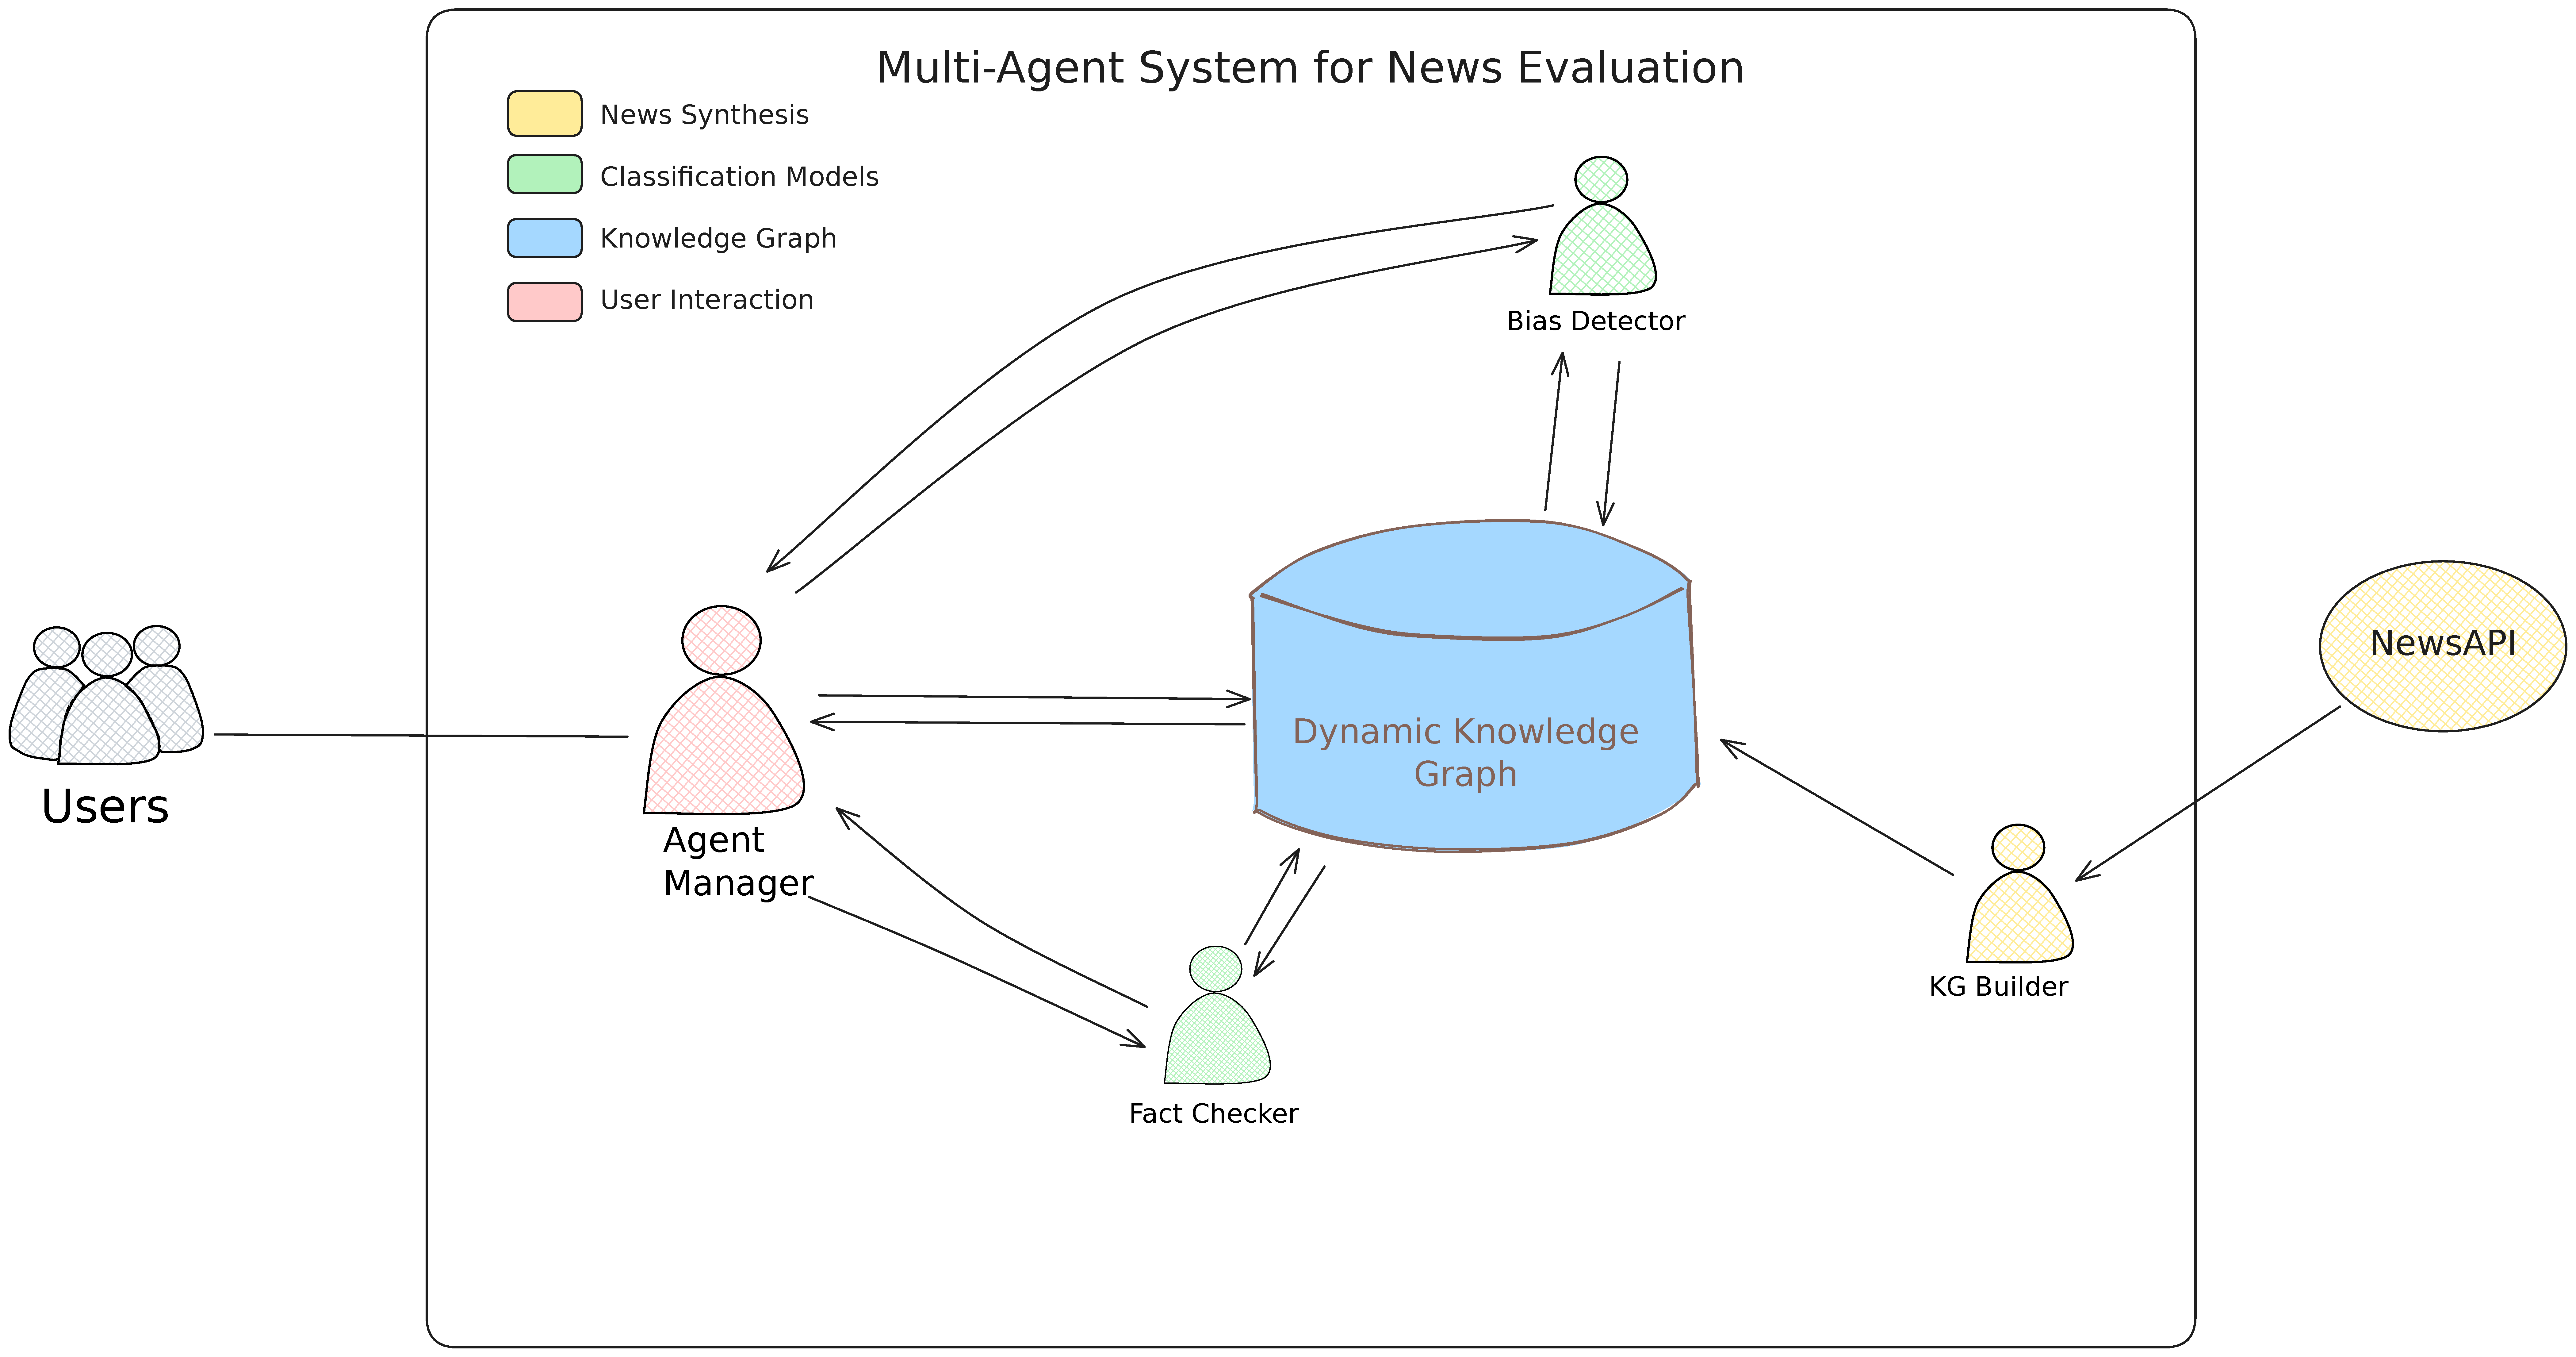
\includegraphics[scale=0.125]{sys_architecture.pdf}
\end{center}
\caption{The system workflow architecture}
\label{setup}
\end{figure}

The system has three main paths in order to provide robust capability in news evaluation. Figure 1 shows the  The main path consists of fetching news from the NewsAPI and building the KG. The user interacts with the chatbot, and the agent manager directs queries to the most appropriate agent or the KG itself. Each agent operates independently and directly with the KG.

The next two paths are specific to the Fact Checker and Bias Detector. They independently receive queries and interact directly with the KG to provide a response. The decision-making workflow is shown in Algorithm 1.

\renewcommand{\thealgocf}{1}
\begin{algorithm}[H]
\caption{System Workflow Design}
\KwIn{User request (news search, bias detection, or fact-checking)}
\KwOut{Processed output based on selected path}

\SetKwBlock{MainPath}{Main Workflow Paths}{end}
\SetKwBlock{FactPath}{Fact Check Path}{end}
\SetKwBlock{BiasPath}{Bias Analysis Path}{end}

\MainPath{
    1. KG Builder fetches news from NewsAPI and updates the Knowledge Graph\;
    2. Bias Detector and Fact Checker interact directly with the Knowledge Graph\;
    3. Agent Manager handles user interactions and can trigger any of the above processes\;
    4. Each Agent operates independently, interacting via the Knowledge Graph\;
}

\FactPath{
    1. Route directly to the Fact Checker Agent\;
    2. Triggered when user provides a specific claim for verification\;
    3. Bypasses News Collection and Bias Analysis\;
}

\BiasPath{
    1. Route directly to the Bias Analyzer Agent\;
    2. Triggered when user wants to analyze article bias\;
    3. Bypasses News Collection\;
}

\Return{Output generated by selected agent(s) via Knowledge Graph}
\caption{System decision making workflow for processing user queries.}
\end{algorithm}

This architecture facilitates flexibility as components do not directly rely on one another, but each agent collaborates independently via the shared knowledge graph. 

\subsubsection{Agent Manager Design}
The agent manager controls the operation and overall workflow in the architecture effectively. The manger coordinates to which agent, if any, user queries should be sent and ensures the response is returned back to the user.  
\renewcommand{\thealgocf}{2}
\begin{algorithm}[H]
\caption{Agent Manager Path Determination}
\KwIn{User input query}
\KwOut{Selected processing path}

\SetKwFunction{FactCheck}{FactCheckPath}
\SetKwFunction{Bias}{BiasPath}
\SetKwFunction{Full}{FullWorkflow}

\SetKwBlock{Manager}{Agent Manager Workflow}{end}

\Manager{
    1. Receive user input\;
    2. Analyze input to determine intent\;
    
    \If{input contains a claim}{
        \FactCheck{}\;
    }
    \ElseIf{input is bias query}{
        \Bias{}\;
    }
    \Else{
        \Full{}\;
    }

    3. Route request to the appropriate agent(s)\;
    4. Return results to the user\;
}

\SetKwBlock{FactCheckPath}{\FactCheck: Fact Check Path}{end}
\FactCheckPath{
    Direct input to Fact Checker Agent\;
    Skip news fetching and bias detection\;
}

\SetKwBlock{BiasPath}{\Bias: Bias Analysis Path}{end}
\BiasPath{
    Direct input to Bias Detection Agent\;
    Skip news fetching and fact checking\;
}

\SetKwBlock{FullWorkflow}{\Full: Full Path}{end}
\FullWorkflow{
    Trigger news fetching via KG Builder\;
    Then run Bias Detection and Fact Checking in sequence\;
}

\end{algorithm}


\subsection{Fact Checker Agent Design and Implementation}
The agent fact-checker is designed to verify the truthfulness of user-provided claims by using the shared KG and LLM—Claude 3.5 Sonnet’s—reasoning abilities. Its implementation follows a pipeline that combines structured retrieval and natural language analysis.

\begin{enumerate}

    \item Claim parsing: Upon submission of a claim for verification by a user. fact-checker initially analyzes the claim utilizing LangChain’s graph transformer to discern its essential components and produce triplets.
    
    \item Query KG: The agent then queries the KG using a Cypher query template and the extracted triplets to find similar facts or context. Any information that supports or refutes the claim is retrieved.
    
    \item Prompt Construction: The fact checker builds a prompt for the LLM that incorporates the original claim and the supporting evidence from the graph. In the prompt, LLM is directed to prioritize the information provided by the KG over its internal information to weigh the facts from the KG.
    
    \item LLM Analysis and Verdict: The LLM processes the prompt and weighs the claim against the evidence. The fact checker determines whether the claim contradicts the evidence or aligns with it  and produces a true/false response and provides the reasoning for its determination
 

\end{enumerate}

The fact-checker agent effectively operates as the interface between the structured information in the KG and the unstructured reasoning of the LLM.  In its current implementation, the KG is the primary source of evidence for the agent. By design, this agent can also be extensible to search the web for information that is not in the KG, but this was not included in this initial work. 

\subsection{Bias Detection Agent Implementation}
The Bias Detection Agent focuses on determining the presence and lean of political bias in a provided news article by comparing it with other coverage of the same subject in the KG. Its implementation uses the KG as a basis for contextual comparisons, using other articles as a baseline to judge the slant of the target article.

\begin{enumerate}
\item Article Parsing: Upon receiving a news article to analyze, the agent leverages LangChain’s Graph Transformer to extract the key topics, entities, and relationships in the article and produce triplets.
    
    \item Bias Retrieval from KG: The agent queries the KG for the most structurally similar article in the KG, meaning the identified article shares the most nodes and edges as the provided article. The agent retrieves only the bias of the most structurally similar article and passes that to the LLM.
    
    \item Bias Prompt Construction: The Bias Detection Agent assembles a prompt using the provided article contents, the bias of the most similar KG article, and the shared entities between the articles. The LLM is prompted to use the evidence provided by the similar article as a clue but also to evaluate the article for specific tone or word choices that may indicate a bias.
    
    \item  LLM Bias Classification: The LLM analyzes the prompt, provides a “Left,” “Center,” or “Right” verdict, and offers good reasoning for this determination capability.
\end{enumerate}

An article by itself may be difficult to determine the bias, but by providing structurally similar bias in articles and the shared entities as a clue, the LLM can make a better determination of the provided article’s. The KG provides key context that an LLM alone will likely miss.

\subsection{Knowledge Graph Components}
In this section, we describe how the KG is built, its schema, and how agents interact with it so it can be the central shared memory in the multi-agent system. Figure 2 shows a portion of an example KG that uses matching nodes and relationships as the one used for this effort. 
\begin{figure}[h!]
\begin{center}

\hspace*{-2cm}    
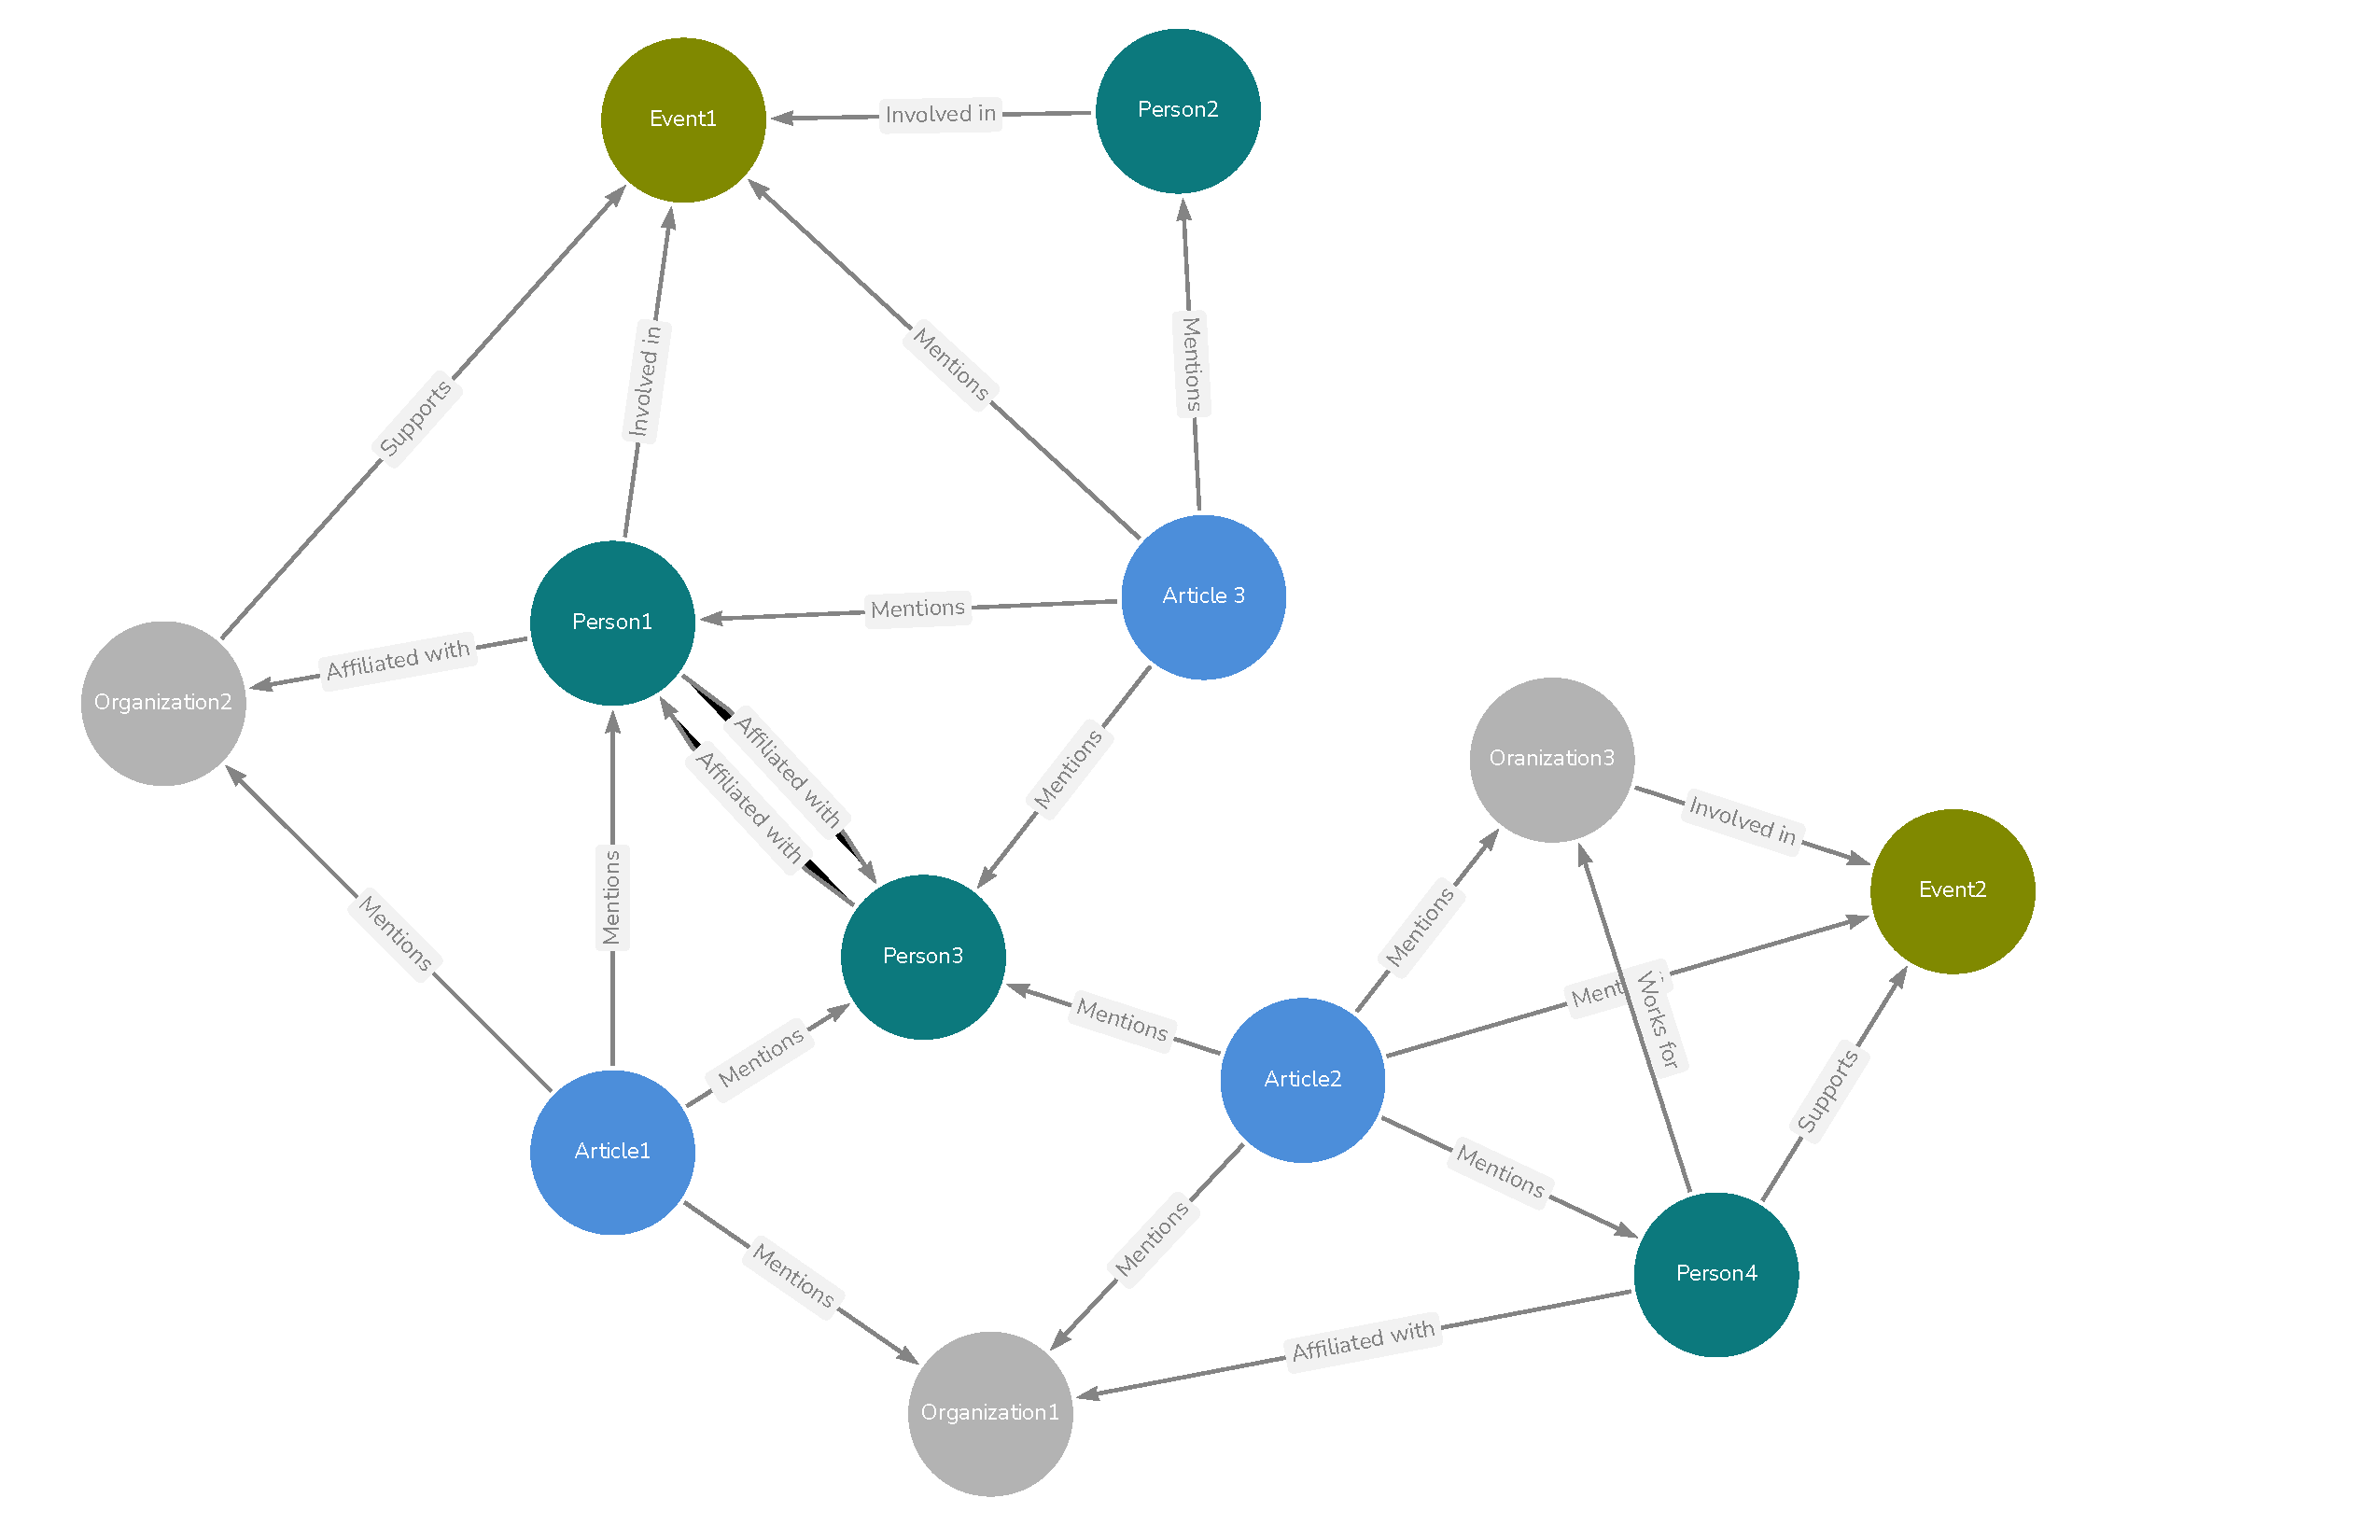
\includegraphics[scale=0.5]{graph_schema.pdf}

\end{center}
\caption{An example portion of the knowledge graph schema. Blue nodes represent news articles in the corpus from which the other entity nodes have been extracted. Several articles can be related to similar entities enabling complex relationships between the nodes.
}
\label{setup}
\end{figure}

\subsubsection{KG Builder}

The KG Builder module constructs and updates the knowledge graph using raw textual inputs. The KG Builder utilizes LangChain’s LLM Graph Transformer and Claude 3.5 Sonnet to convert unstructured news article text collected from the NewsAPI into structured graph data (Figure 2). The builder identifies entities and relationships from news articles and structures them into triplets that can be added to the KG.
The KG builder is configured to allow certain nodes and relationships relevant to U.S. political news to ensure that the KG stays relevant to the scope of this effort, maintains a structured format, and reduces noise in the content. The builder functions also include methods for avoiding duplicate nodes when the same entity appears. The Graph Transformer also creates additional relationships in the KG that are not specified in the schema. This results in a robust, structured, and interconnected knowledge base for the news articles that our agents can access to address user queries.

\subsubsection{Knowledge Representation Schema}

The schema of the news KG is designed to capture the important elements of the news content and their interconnections. The KG is centered around news article nodes that connect to the other types of nodes in the KG. This approach allows us to make queries traceable to news articles and better understand complex relationships in the data. We define several types of nodes and edges:

\renewcommand{\thealgocf}{3}
\begin{algorithm}[h!]
\caption{Initialize News Knowledge Graph Schema}
\KwIn{News article corpus}
\KwOut{Structured Knowledge Graph (KG)}

\SetKwBlock{Define}{Define}{end}

\Define (\textbf{Nodes})
{

    {\textbf{Article}\;
    \textbf{Person}\;
    \textbf{Organization}\;
    \textbf{Event}\;
    \textbf{Policy}\;
    \textbf{Issue}\;
    \textbf{Location}\;
    \textbf{Election}\;
    \textbf{Bill}\;
    \textbf{Vote}\;
    \textbf{Speech}\;
    \textbf{Alliance}\;}
}

\Define (\textbf{Edge Types})
{
    \textbf{Mentions} (\textit{Article} $\rightarrow$ Any Entity)\;
    \textbf{Affiliated With} (Any Entity $\leftrightarrow$ Any Entity)\;
    \textbf{Participated In} (\textit{Person} $\rightarrow$ \textit{Event})\;
    \textbf{Endorsed} (\textit{Person} $\rightarrow$ \textit{Policy})\;
    \textbf{Sponsored} (\textit{Person} $\rightarrow$ \textit{Bill})\;
    \textbf{Gave Speech} (\textit{Person} $\rightarrow$ \textit{Speech})\;
    \textbf{Involved In} (\textit{Person} $\rightarrow$ \textit{Event})\;
    \textbf{Organized} (\textit{Organization} $\rightarrow$ \textit{Event})\;
    \textbf{Supports} (\textit{Organization} $\rightarrow$ \textit{Policy})\;
    \textbf{Lobbied For} (\textit{Organization} $\rightarrow$ \textit{Bill})\;
    \textbf{Takes Place In} (\textit{Event} $\rightarrow$ \textit{Location})\;
    \textbf{Addresses} (\textit{Policy/Speech} $\rightarrow$ \textit{Issue})\;
    \textbf{Decided By} (\textit{Bill} $\rightarrow$ \textit{Vote/Organization/Person})\;
    \textbf{Includes} (Any Entity $\rightarrow$ Any Entity)\;
}

\Return{Initialized KG Schema}

\end{algorithm}


\subsection{ Knowledge Graph Query Mechanisms}
A user interfaces with our system using an LLM chatbot. Based on the user input, the chatbot will interact with the KG directly or pass the interaction to another agent. The agents then generate the Cypher query by extracting key information from the user message in the form of nodes and relationships that align to those present in the KG. The extracted elements are formatted into  pre-built Cypher templates to interact directly with the KG. Once a query is executed the reseult are provided in the form of triplets back to the agent. Through a combination of Cypher querying and LLM-driven element extraction, the agents can flexibly pull the information they need from the graph.
 
\subsection{Knowledge Sharing Protocol}
A key aspect of the system architecture is that the KG serves as a shared memory space for all agents. This sharing protocol ensures that updates to the KG and queries against it happen in a coordinated fashion so that each agent has a consistent and current view of the knowledge. Each agent, whether it’s the KG Builder, the Fact Checker, the Bias Detector, or the Chatbot, interacts with the KG through a defined interface through the Neo4j API.

Currently, the KG Builder helps to write into the KG, and as soon as it makes changes or updates the KG, the other agents all have access to the new information. This is a benefit of using the shared memory; if one agent makes an update or change, all other agents will have immediate access to that information.

\subsection{Implementation Details}
\subsubsection{Technologies and Frameworks}
The multi-agent system was implemented using a modern technology stack centered around:
\begin{enumerate}
    \item Core Language used in the development: Python 3.12.3 for all components
    \item Large Language Model: AWS Bedrock Claude 3.5 Sonnet v2 for powering the multi-agent capabilities.
\item Knowledge Graph: Neo4j graph database for storing and querying news data.  
\item Machine Learning Libraries: LangChain as a multi-agent framework and for agent management, LangChain-Neo4j for graph database-agent interactions, LangChain-experimental for graph transformer tools.
\end{enumerate}

\subsection{Limitations of Current Approach}
Even though the system is successful, the approach has key limitations that, if addressed, can further improve the capability:
\begin{enumerate}
    \item Entity Recognition: The LLMGraphTransformer sometimes struggles identifying the most influential entities and relationships in an article. Tuning the LLMGraphTransformer through prompting and KG design is a key to successful deployment. If under-restricted, the LLMGraphTransformer will extract every detail and relationship, generating significant noise in the KG. If over-restricted, the KG will lose effective context for successful implementation.
    \item Context Window Constraints: Claude 3.5’s token limits restrict the amount of contextual information that can be processed in single requests. This particularly affects triplet extraction from long-form articles. There may be important details that are not incorporated into the KG. This can be mitigated with chunking techniques but was not implemented in this project. 
\end{enumerate}

\section{System Testing and Evaluation}
\subsection{Testing Methodology}
Our testing strategy employs a comprehensive evaluation framework designed to assess both component-level functionality and system-wide performance. The strategy follows a dual approach:
\subsubsection{Isolated Component Evaluation: Unit Test}
Individual agents and components of the knowledge graph are tested separately to ensure that they meet functional requirements and performance benchmarks. The dual layer approach used is the use of mock to test component logic in isolation and its fast, deterministic, and does not require external services. Serves as a primary testing layer for development and CI/CD. The automated uint- test suites for:
\begin{enumerate}
    \item Knowledge graph operations (article retrieval, bias assessment, fact verification)
    \item Fact checker functionality (entity extraction, claim verification)
    \item Bias analyzer performance (bias detection accuracy, context utilization)

\end{enumerate}

\subsubsection{End-to-End System Testing: Integration Test}
The complete system is evaluated using real-world data to measure overall effectiveness and validate information flow. We conducted end-to-end testing using a corpus of political news articles. The testing and evaluation focused on:
\begin{enumerate}
    \item System response quality
    \item Processing efficiency
    \item Knowledge graph utilization
    \item Error resilience 
\end{enumerate}

\subsubsection{User Interface Implementation}
A user interface was developed using Streamlit. This gives a user the ability to interact with the system in natural language and get back a natural language response for bias and fact check results. 

\subsection{Evaluation Metrics}
\subsubsection{Accuracy, Precision, Recall}
In this research evaluation for multi-agent system, we employed standard classification metrics that are particularly appropriate for tasks involving class imbalance:
\begin{itemize}
    \item \textbf{Precision} measures the proportion of correct identifications (true positives divided by all positive predictions). This metric was especially important for fact-checking, where false accusations of misinformation could damage credibility. For bias detection, precision indicates how reliably the system can identify specific bias categories.
    \item \textbf{Recall} (also known as sensitivity) measures the proportion of actual positives correctly identified (true positives divided by all actual positives). This was critical for fact-checking to ensure truthful claims weren’t incorrectly flagged as false, despite our dataset’s significant class imbalance.
    \item \textbf{F1-score} represents the harmonic mean of precision and recall, providing a balanced measure that considers both false positives and false negatives. This was particularly valuable for our imbalanced fact-checking dataset 
    \item \textbf{Accuracy} measures the proportion of correct predictions among the total number of cases evaluated. While useful as an overall metric, we supplemented it with balanced accuracy for the bias detection task to account for class imbalance.
\end{itemize}

\subsubsection{System-specific Performance Metrics}
In addition to standard classification metrics, we employed specialized metrics tailored to our specific evaluation tasks: 
\begin{itemize}
    \item Balanced accuracy accounts for class imbalance by calculating the average of recall obtained on each class. This metric helps us understand the performance of our bias detection across Left, Center, and Right regardless of their proportion in the dataset. 
    \item  Cohen’s Kappa measures inter-rater agreement while accounting for chance agreement. It is valuable in our bias detection for assessing how closely our system’s classifications are aligned with human annotations beyond random agreement. 
    \item Matthews Correlation Coefficient (MCC) provides a balanced measure for binary and multiclass classification problems even with class imbalance. This metric was useful for bias detection, offering a comprehensive evaluation of classification performance. 
    \item Weighted F1 calculates the average F1 score weighted by number of instances for each class, providing a more representative measure of overall performance across imbalanced classes.
\end{itemize}

\subsection{Experimental Setup}
\subsubsection{Test Data Characteristics}
For fact-checking evaluation, we compiled a benchmark dataset by scraping Media Bias/Fact Check (MBFC)’s Daily Fact Checks from February to April 2025. Table 1 shows the breakdown of the labels for claims that were collected. Each claim’s label corresponds to the verdict reported by MBFC, providing ground-truth annotations for evaluating our system’s fact checking performance. Before preprocessing additional labels "Misleading" and "Missing" were found in the dataset but were removed for our evaluation. The resulting dataset comprises 210 claims, with 40 (19\%) labeled as "True" and 170 (81\%) labeled as "False," indicating a notable class imbalance. 
\begin{table}[H]
\begin{center}
\begin{tabular}{llll}
\hline
\multicolumn{4}{c}{Fact Check Data Preprocessing}                     \\
                & \multicolumn{2}{l}{Before}       & After            \\ \hline
False           & \multicolumn{2}{l}{170 (74.2\%)} & 170 (81.9\%)     \\
Misleading& \multicolumn{2}{l}{4 (1.7\%)}    & 0 (0.0\%)        \\
Missing         & \multicolumn{2}{l}{15 (6.6\%)}   & 0 (0.0\%)        \\
True& \multicolumn{2}{l}{40 (6.6\%)}   & 40 (19.0\%)      \\ \hline
\end{tabular}
\caption{Fact checking dataset before and after data pre-processing}
\end{center}
\label{tab:my_table}
\end{table}

For bias detection, we compiled an evaluation corpus of 222 news articles,  labeled with its source's AllSides bias rating. Table 2 shows the dataset before and after pre-processing. Articles labeled "Lean Left" were categorized as "Left" for this evaluation. The resulting dataset used for evaluation contained a only "Left", "Center", and "Right" bias labels. This was used as a ground truth when evaluating the system's bias detection performance. 
\begin{table}[H]
\begin{center}
\begin{tabular}{lll}
\hline
\multicolumn{3}{c}{Bias Data Preprocessing} \\
            & Before        & After         \\ \hline
Center      & 17 (7.7\%)    & 17 (7.7\%)    \\
Lean Left   & 38 (17.1\%)   & 0 (0.0\%)     \\
Left        & 93 (41.9\%)   & 131 (59.0\%)  \\
Right       & 74 (33.3\%)   & 74 (33.3\%)   \\ \hline
\end{tabular}
\caption{Bias dataset before and after data pre-processing}
\label{tab:my_table}
\end{center}
\end{table}

The articles and claims in the evaluation datasets were not present in the knowledge graph. However, the same news sources were used for the bias evaluation dataset and the knowledge graph due to availability of full article text from the NewsAPI. This separation ensures an unbiased assessment of unseen data, validating that the system’s performance is not inflated by data leakage.

\subsubsection{Comparative Systems}

To evaluate the impact of knowledge graph integration, we implemented two system configurations:
\begin{enumerate}
    \item LLM-only: A baseline system using AWS Bedrock Claude 3.5 Sonnet v2 with direct prompting but no knowledge graph integration. 
    \item LLM+KG: Our complete multi-agent system with the same AWS Bedrock Claude 3.5 Sonnet v2 model.
\end{enumerate}

Both systems employed identical prompt templates and preprocessing procedures to guarantee an equitable comparison This configuration serves as a control to isolate the effect of the knowledge graph.

\subsubsection{Evaluation Parameters}
The evaluation was conducted with the following parameters:
\begin{enumerate}
    \item LLM Temperature: 0.2 for all queries 
    \item Maximum Token Limit: 4,096 tokens per request
    \item Knowledge Graph Query Depth: Maximum 2-hop traversal for related entities
    \item Bias Categories: Three-class classification (Left, Center, Right)
    \item Fact-Check Categories: Binary classification (True, False) 
    \item Testing Environment: Isolated environment with controlled network access
    \item Evaluation Mode: Batch processing of all test instances with results logged for analysis
\end{enumerate}
For each test case, we recorded the system’s prediction and reasoning for the prediction. 

\section{Results}
\subsection{Quantitative Performance Analysis}
\subsubsection{Comparative Performance Metrics}

\textbf{Fact Checking Results} 

\textbf{LM-Only Performance}: LLM-Only Performance The LLM-only model achieved an overall accuracy (microaverage F1 score) of 0.77 (Table 3). Although it performed well in the majority class (False) with a precision of 0.75 and recall of 0.96 (F1 score: 0.84), its performance in the minority True class was notably poor. The recall for True claims was only 0.07, resulting in a low F1 score of 0.14, highlighting the model’s tendency to favor the dominant class and ignore minority examples.
 
\textbf{LLM + Knowledge Graph Performance}: In contrast, the model enhanced with KG context showed notable improvements across nearly all metrics (Figure 3), particularly in its ability to handle the underrepresented True class. The recall for True claims increased substantially from 0.07 to 0.25, and the corresponding F1-score improved from 0.14 to 0.38. The overall microaverage F1 score increased to 0.82, and the macroaverage F1 score –which gives equal weight to both classes –rose from 0.49 to 0.63, a 14-point gain.


\begin{table}[H]
\begin{center}
\begin{tabular}{lcccc}
\hline
\multicolumn{5}{c}{LLM-Only}                                                                                                               \\
                 & \multicolumn{1}{l}{Precision} & \multicolumn{1}{l}{Recall} & \multicolumn{1}{l}{F1-score} & \multicolumn{1}{l}{Support} \\ \hline
True             & 0.75                          & 0.07                       & 0.14                         & 40                          \\
False            & 0.75                          & 0.96                       & 0.84                         & 170                         \\
Micro Average    & 0.75                          & 0.79                       & 0.77                         & 210                         \\
Macro Average    & 0.75                          & 0.52                       & 0.49                         & 210                         \\
Weighted Average & 0.75                          & 0.79                       & 0.71                         & 210                         \\ \hline
\multicolumn{5}{l}{LLM + KG}                                                                                                               \\ \hline
                 & \multicolumn{1}{l}{Precision} & \multicolumn{1}{l}{Recall} & \multicolumn{1}{l}{F1-score} & \multicolumn{1}{l}{Support} \\
True             & 0.77                          & 0.25                       & 0.38                         & 40                          \\
False            & 0.78                          & 0.99                       & 0.88                         & 170                         \\
Micro Average    & 0.78                          & 0.85                       & 0.82                         & 210                         \\
Macro Average    & 0.78                          & 0.62                       & 0.63                         & 210                         \\
Weighted Average & 0.78                          & 0.85                       & 0.78                         & 210                         \\ \hline
\end{tabular}
\caption{Comparison of metrics for fact-checking evaluation between the benchmark LLM and the LLM+KG system.}
\label{tab:my_table}
\end{center}
\end{table}

\begin{figure}[H]
\begin{center}
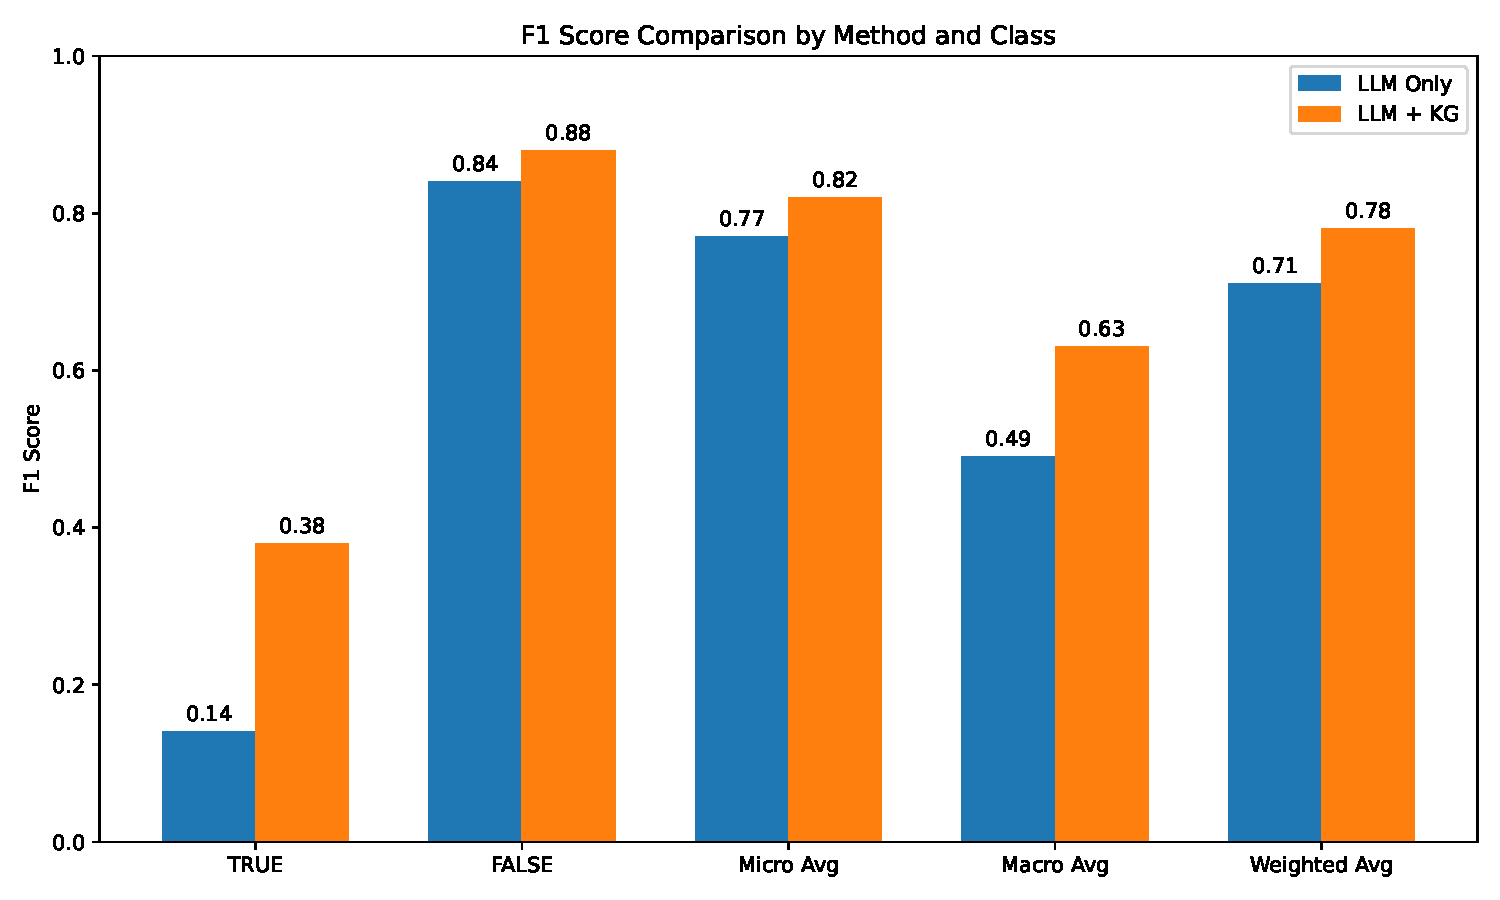
\includegraphics[scale=0.3]{factcheck-results.pdf}
\end{center}
\caption{Comparison of F1 score by method and class. This shows the KG improves the LLM's fact-checking ability across all metrics.}
\label{fig:factcheck-results}
\end{figure}
This shows that incorporating structured knowledge not only improves the overall classification accuracy but also significantly improves the model’s sensitivity to minority class instances, a key concern in unbalanced datasets. The weighted average F1 score increased from 0.71 to 0.78, reinforcing that the KG-augmented model maintained strong performance in the dominant class while improving minority class detection.


\subsubsection{Bias Detection Results}
\textbf{LLM-Only Performance}: The LLM-only system achieved a balanced accuracy of 0.735 (Table 4), a Cohen’s kappa of 0.488, and a macro F1 score of 0.615. These results indicate agreement with ground truth and a limited ability to handle the minority class. The Matthews correlation coefficient (MCC) of 0.574 and the weighted F1 score of 0.705 further demonstrate that the model performed better in major classes but lacked generalization across all classes.
 
\textbf{LLM + Knowledge Graph Performance}: The model enhanced with the KG context showed significant performance gains across all metrics (Figure 4). The balance accuracy improved to 0.823, indicating a much better handling of class imbalance. Cohen’s kappa increased to 0.745, suggesting strong agreement beyond chance. The macro F1 score rose to 0.76, indicating enhanced performance in minority classes, including Center. The MCC increased to 0.759, and the weighted F1 score attained 0.877, indicating that the model reliably assigned bias labels with greater accuracy and equity across all class distributions. 


\begin{table}[H]
\begin{tabular}{@{}lccccc@{}}
\toprule
         & \multicolumn{5}{c}{Bias Detection Performance Metric}                                                                                                                                                \\
         & \multicolumn{1}{l}{Balanced   Accuracy} & \multicolumn{1}{l}{Cohen Kappa} & \multicolumn{1}{l}{Macro F1} & \multicolumn{1}{l}{Matthews Correlation} & \multicolumn{1}{l}{Weighted F1} \\ \midrule
LLM-Only & 0.735                                   & 0.488                           & 0.615                        & 0.574                                    & 0.705                           \\
LLM-KG   & 0.823                                   & 0.745                           & 0.76                         & 0.759                                    & 0.877                           \\ \bottomrule
\end{tabular}
\caption{Comparison of bias detection results between the LLM-only benchmark and the LLM+KG system.}
\label{tab:my_table}
\end{table}


\begin{figure}[H]
\begin{center}
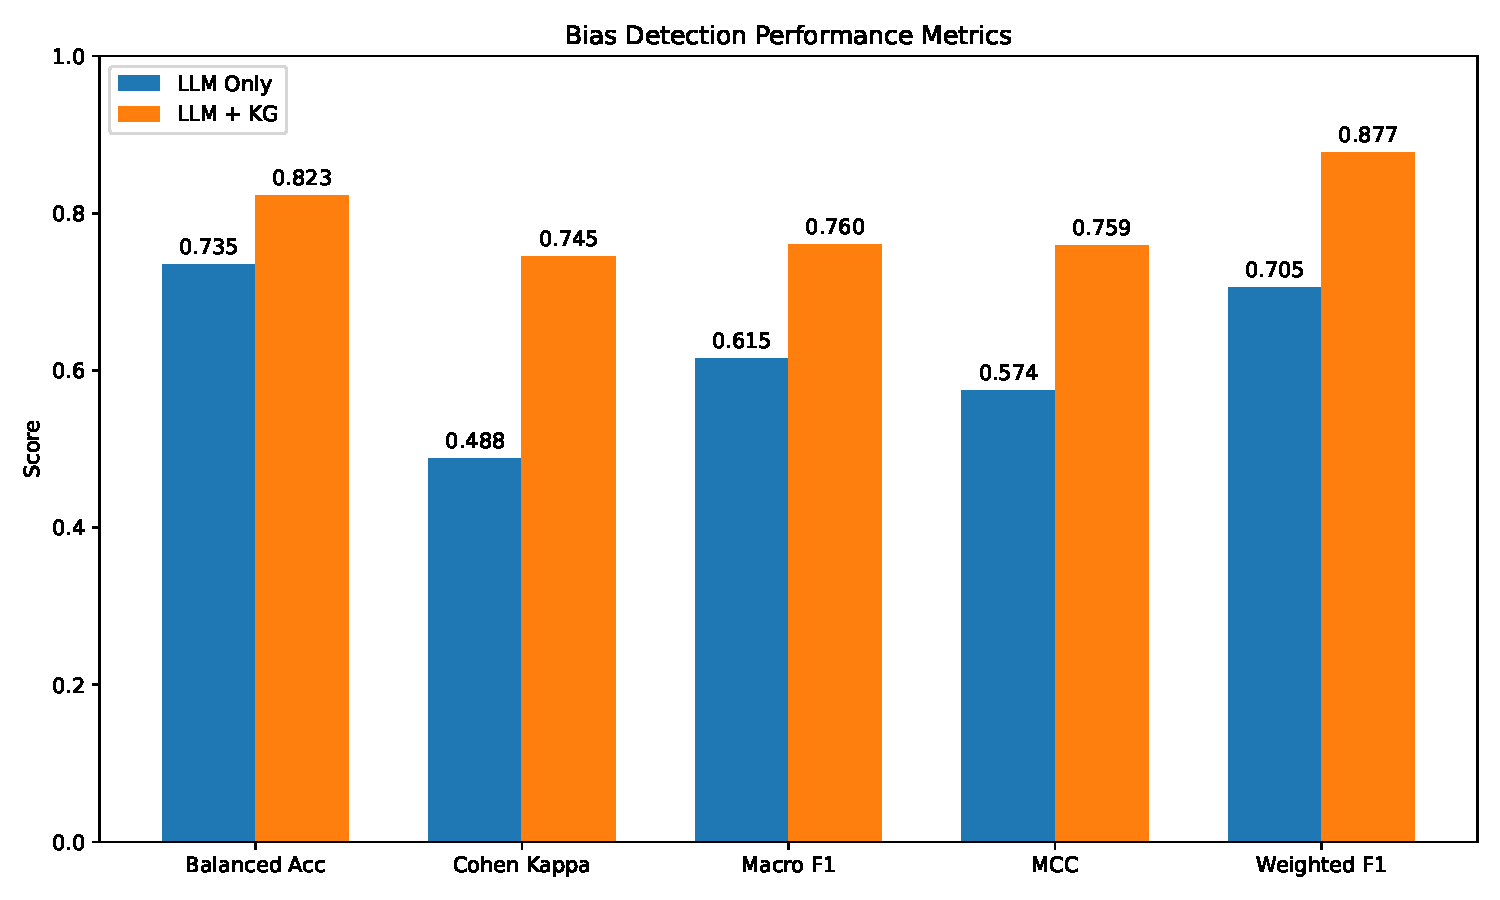
\includegraphics[scale=0.3]{bias-results.pdf}
\end{center}
\caption{The results of bias detection with the LLM+KG against the benchmark of just the LLM.}
\label{fig:bias-results}
\end{figure}
These findings indicate that the integration of a knowledge graph significantly enhances the robustness and fairness of LLM-based bias detection models, especially in imbalanced multiclass settings. 


\subsection{Qualitative Analysis}

\subsubsection{Error Analysis}
The LLM-only configuration showed an extremely low true-claim recall (0.07), indicating that it missed most factual statements. The KG integration improved this to 0.25, though it is still showing room for improvement. For bias detection, the LLM+KG configuration showed the greatest improvement in Matthews correlation coefficient (from 0.574 to 0.759), indicating a better overall classification across all bias categories.


\section{Discussion}
\subsection{Interpretation of Results}
The experiment performance improvements support our research hypothesis and objectives that integrating  KGs with multi-agent LLM architectures creates significant improvements and benefits. The KG integration particularly improved:
\begin{enumerate}
    \item Balanced accuracy (12\% improvement) and Cohen’s kappa (0.488 to 0.745, a 53\% increase) for bias detection
    \item True claim recall in fact-checking (0.07 to 0.25, a 257\% increase)
\end{enumerate}

These improvements indicate that the use of KG provides critical contextual information that LLMs lack when operating independently.

\subsection{Comparison with Existing Systems}

Our experiment results demonstrate significant improvements over LLM-only approaches for bias detection and fact-checking. The integrated system achieves 0.823 balanced accuracy for bias detection, compared to 0.735 for the LLM-only configuration. This is a significant improvement and encourages further exploration. 
While improvement in fact-checking metrics are modest, the substantial increase in true claim recall (0.07 to 0.25) suggests better identification of verifiable facts. This may be mitigated with more robust news collection but remains an area of interest for future study.

\subsection{Limitations Discovered During Evaluation}
The primary observed limitation is that the system occasionally struggles with emerging political narratives not yet well represented in the knowledge graph. If only a few articles about a specific topic are present in the KG, they may have an outsized influence and the system may present a skewed contextual information rather than a balanced view. 

\subsection{Implications for News Evaluation Research}
In future research, These findings suggest news evaluation should further explore approaches to bias detection and fact-checking that combine LLMs with KGs for structured contextual information. The observed significant improvements across all metrics make this research experimental approach is a good candidate to augment fact check and editorial teams.

\section{Conclusion}
\subsection{ Summary of Contributions}
This research presents two important contributions: (1) improved multi-agent architecture combining LLM capabilities with a shared KG for news evaluation and (2) evidence of significant performance improvements across all metrics for bias detection and modest performance improvement in fact-checking. 

\subsection{Achievement of Research Objectives}
Our research successfully shows the effectiveness of integrated architectures and the value of providing structured contextual knowledge to LLM-based systems through the use of KG. We showed measured performance improvement between multi-agent systems with and without KG integration.

\subsection{Practical Applications}
The developed system has immediate real-world practical applications in journalistic industrial workflows, provides valuable educational contexts, and media literacy programs. News organizations and outlets can implement this architecture to provide rapid fact-checking and bias analysis, while media experts and educators can use it to teach critical media analysis skills.


\section{Future Work}

\subsection{Architectural Improvements}
Future research should primarily focus on optimizing agent communication protocols based on performance feedback. The introduction of additional agents that write to the KG can offer an aspect of continued learning even when the news corpus is not being updated. Having agents annotate the KG will provide additional bias or fact content that can be considered when making evaluations. 

\subsection{Knowledge Graph Enhancements}
Other future research could be the inclusion of vector embeddings into the KG such as GraphRAG can provide another layer of capturing contextual information for agents to use to improve news evaluations. Adding a temporal element to the KG to weigh emerging news stories should also be explored in future work.

\subsection{Additional Agent Types}
Additionally, we proposed the inclusion of the new agents to include rhetorical analysis specialists, source credibility evaluators, and narrative frame detectors. These specific specialized agents would further enhance the system’s overall analytical capabilities and provide a more comprehensive news evaluation in bias and fact-checking.

\subsection{Real-World Deployment Considerations}
The real-world consideration in production deployment requires addressing scalability challenges, implementing robust error-handling mechanisms, and developing user interfaces based on different stakeholder groups (journalists, educators, researchers). In addition, there should be ethical considerations regarding transparency, accountability, and potential misuse must be carefully addressed through established governance policy guidelines.
 
\subsection{Full System Documentation}
Technical documentation for this project and the software developed is available at:  
\href{https://modupeolawuraola.github.io/Multi-Agent-System-with-Knowledge-Sharing-For-News-Evaluation/architecture.html}{github.io/Multi-Agent-System-with-Knowledge-Sharing-For-News-Evaluation}.

\bibliographystyle{unsrt}
\bibliography{references}
\end{document}